\documentclass[border=8pt]{standalone}
\usepackage{tikz}
\usepackage{amsmath}
\usetikzlibrary{positioning,arrows.meta,shapes,shadows,fit,backgrounds,calc}

\begin{document}
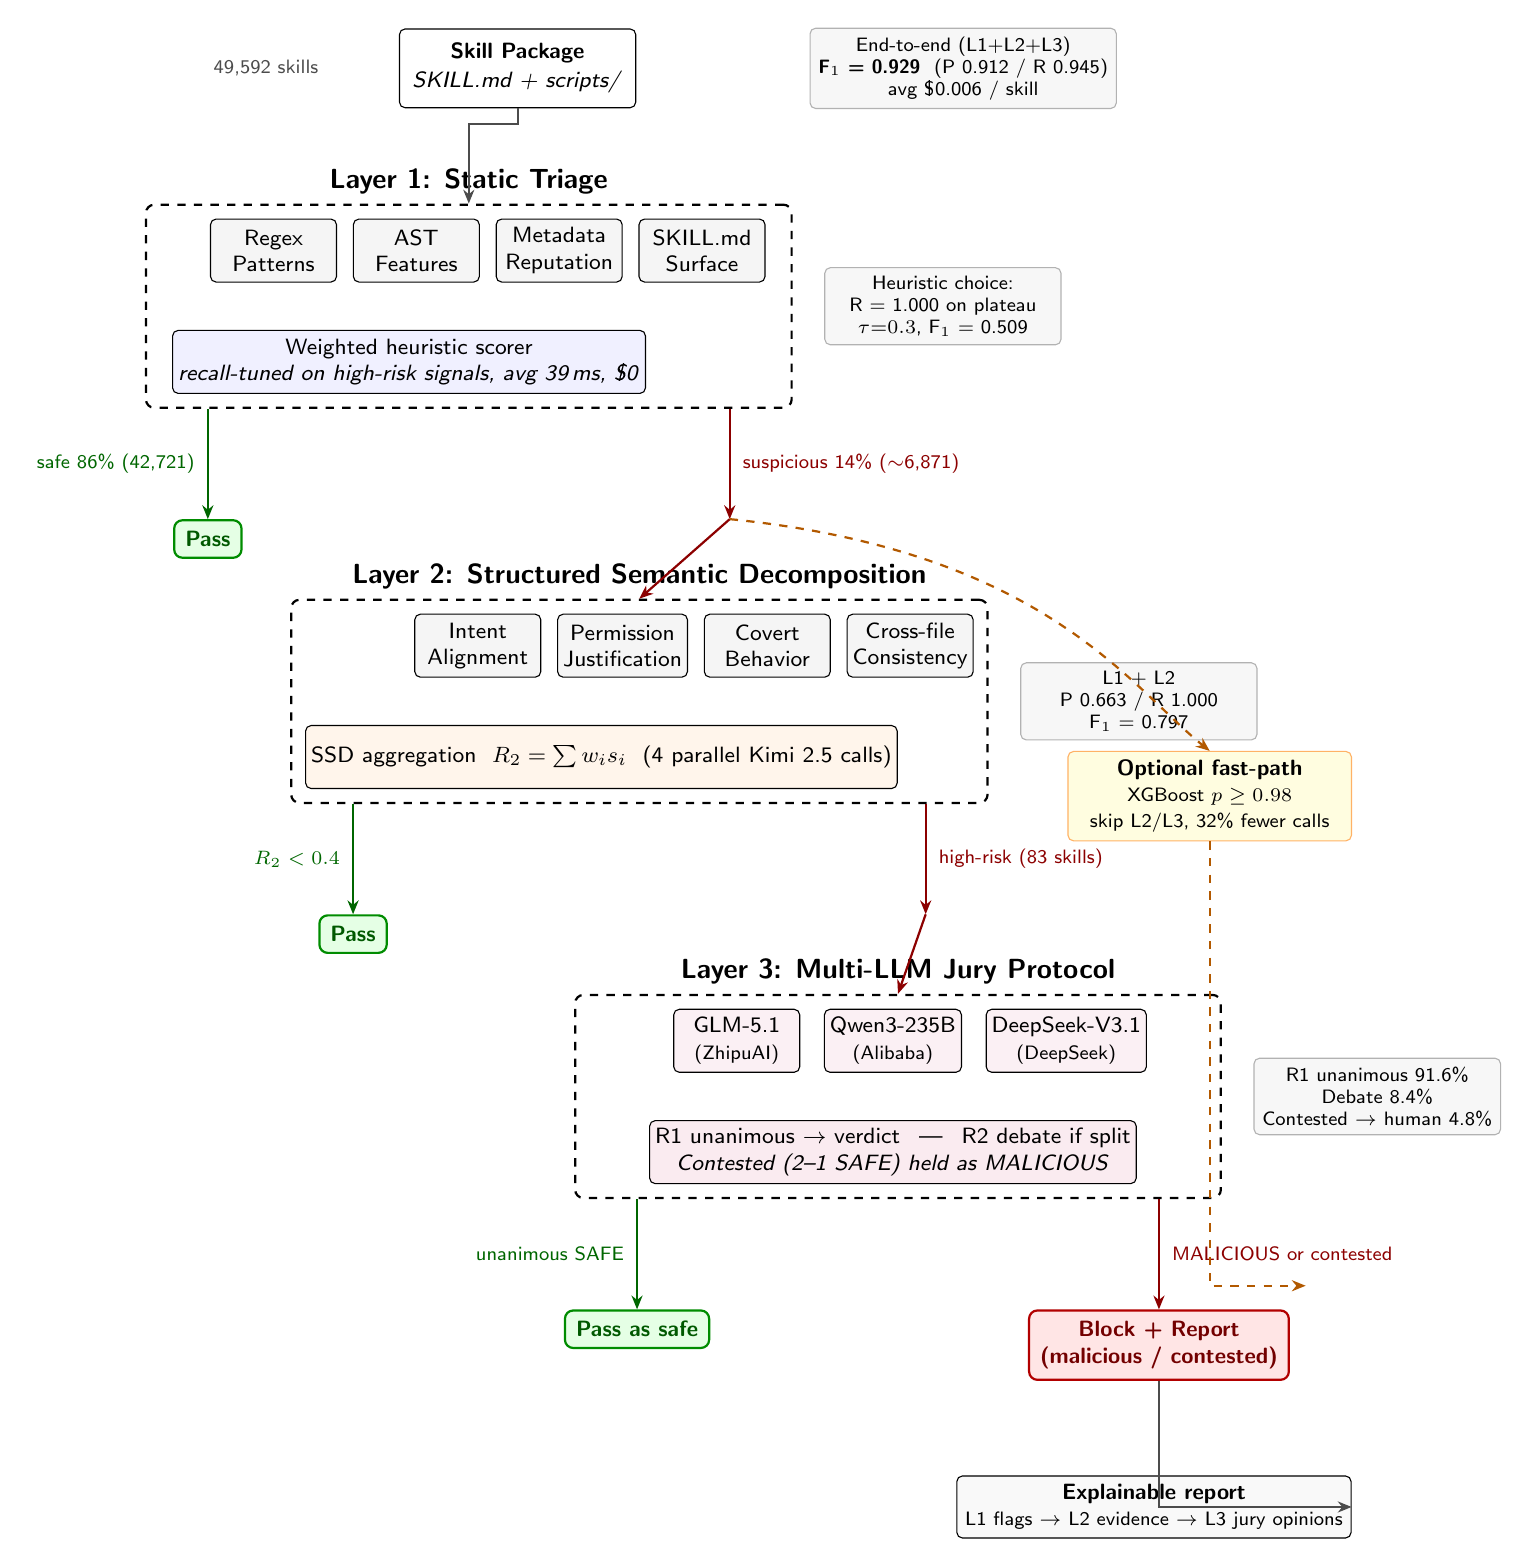
\begin{tikzpicture}[
    font=\sffamily\small,
    >={Stealth[length=5pt,width=4pt]},
    node distance=6mm,
    layerbox/.style={
        draw, thick, rounded corners=3pt, dashed,
        inner sep=5pt, align=center,
        minimum width=82mm,
    },
    submodule/.style={
        draw, rounded corners=2pt, fill=gray!8,
        minimum width=16mm, minimum height=8mm,
        align=center, font=\sffamily\footnotesize,
        inner sep=2pt,
    },
    metric/.style={
        draw=gray!60, fill=gray!6, rounded corners=2pt,
        align=center, font=\sffamily\scriptsize,
        inner sep=3pt, minimum width=30mm,
    },
    tagbox/.style={
        draw, rounded corners=2pt, fill=white,
        align=center, font=\sffamily\footnotesize,
        inner sep=3pt,
    },
    passbox/.style={
        draw=green!55!black, thick, rounded corners=3pt,
        fill=green!10, text=green!35!black,
        align=center, font=\sffamily\bfseries\footnotesize,
        inner sep=4pt,
    },
    blockbox/.style={
        draw=red!70!black, thick, rounded corners=3pt,
        fill=red!10, text=red!45!black,
        align=center, font=\sffamily\bfseries\footnotesize,
        inner sep=4pt,
    },
    flowlabel/.style={
        font=\sffamily\scriptsize,
    },
    safelabel/.style={
        flowlabel, text=green!40!black,
    },
    risklabel/.style={
        flowlabel, text=red!55!black,
    },
    arrow/.style={->, thick, gray!60!black},
]

%==== Top row: Input and headline metric =====================================
\node[tagbox, minimum width=30mm, minimum height=10mm]
    (input) {\textbf{Skill Package}\\[1pt]\textit{SKILL.md + scripts/}};

\node[metric, right=22mm of input, align=center]
    (headline) {End-to-end (L1+L2+L3)\\\textbf{F$_1$ = 0.929} \ (P 0.912 / R 0.945)\\avg \$0.006 / skill};

\node[flowlabel, left=9mm of input, text=gray!60!black]
    (dataset) {49{,}592 skills};

%==== Layer 1 ===================================================================
\node[submodule, below=14mm of input.south, xshift=-31mm] (m_regex)   {Regex\\Patterns};
\node[submodule, right=2mm of m_regex] (m_ast)     {AST\\Features};
\node[submodule, right=2mm of m_ast]   (m_meta)    {Metadata\\Reputation};
\node[submodule, right=2mm of m_meta]  (m_surf)    {SKILL.md\\Surface};

\node[submodule, minimum width=48mm, below=6mm of m_ast.south east,
      xshift=-9mm, fill=blue!6]
    (heur) {Weighted heuristic scorer\\\textit{recall-tuned on high-risk signals, avg 39\,ms, \$0}};

% Draw dashed layer 1 box
\begin{scope}[on background layer]
\node[layerbox, fit=(m_regex)(m_surf)(heur), label={[font=\sffamily\bfseries]above:Layer 1: Static Triage}]
    (L1) {};
\end{scope}

% Layer 1 badge on the right
\node[metric, right=4mm of L1.east, anchor=west, yshift=0mm]
    (L1badge) {Heuristic choice:\\R = 1.000 on plateau\\$\tau{=}0.3$, F$_1$ = 0.509};

% Input arrow to Layer 1
\draw[arrow] (input.south) -- ++(0,-2mm) -| (L1.north);

%==== Branch: safe vs suspicious ============================================
\node[passbox, below=14mm of L1.south west, xshift=8mm] (pass1) {Pass};
\node[coordinate, below=14mm of L1.south east, xshift=-8mm] (susp1) {};

\draw[arrow, green!40!black, thick] (L1.south -| pass1.north) -- (pass1.north)
    node[safelabel, midway, left=1pt] {safe 86\% (42{,}721)};

\draw[arrow, red!55!black, thick] (L1.south -| susp1) -- (susp1)
    node[risklabel, midway, right=1pt] {suspicious 14\% ($\sim$6{,}871)};

%==== Layer 2 ================================================================
\node[submodule, below=12mm of susp1, xshift=-32mm] (t_intent)  {Intent\\Alignment};
\node[submodule, right=2mm of t_intent] (t_perm)    {Permission\\Justification};
\node[submodule, right=2mm of t_perm]   (t_covert)  {Covert\\Behavior};
\node[submodule, right=2mm of t_covert] (t_cross)   {Cross-file\\Consistency};

\node[submodule, minimum width=52mm, below=6mm of t_perm.south east,
      xshift=-11mm, fill=orange!8]
    (ssd) {SSD aggregation \ $R_2 = \sum w_i s_i$ \ (4 parallel Kimi 2.5 calls)};

\begin{scope}[on background layer]
\node[layerbox, fit=(t_intent)(t_cross)(ssd),
      label={[font=\sffamily\bfseries]above:Layer 2: Structured Semantic Decomposition}]
    (L2) {};
\end{scope}

\node[metric, right=4mm of L2.east, anchor=west]
    (L2badge) {L1 + L2\\P 0.663 / R 1.000\\F$_1$ = 0.797};

% Suspicious arrow from L1 to L2
\draw[arrow, red!55!black, thick] (susp1) -- (L2.north);

%==== Branch: L2 pass vs high-risk ==========================================
\node[passbox, below=14mm of L2.south west, xshift=8mm] (pass2) {Pass};
\node[coordinate, below=14mm of L2.south east, xshift=-8mm] (risk2) {};

\draw[arrow, green!40!black, thick] (L2.south -| pass2.north) -- (pass2.north)
    node[safelabel, midway, left=1pt] {$R_2 < 0.4$};

\draw[arrow, red!55!black, thick] (L2.south -| risk2) -- (risk2)
    node[risklabel, midway, right=1pt] {high-risk (83 skills)};

%==== Layer 3 ================================================================
\node[submodule, below=12mm of risk2, xshift=-24mm, fill=purple!6]  (j_glm)   {GLM-5.1\\\scriptsize(ZhipuAI)};
\node[submodule, right=3mm of j_glm, fill=purple!6] (j_qwen)  {Qwen3-235B\\\scriptsize(Alibaba)};
\node[submodule, right=3mm of j_qwen, fill=purple!6] (j_ds)   {DeepSeek-V3.1\\\scriptsize(DeepSeek)};

\node[submodule, minimum width=56mm, below=6mm of j_qwen.south,
      xshift=0mm, fill=purple!8]
    (policy) {R1 unanimous $\to$ verdict \hspace{4pt}|\hspace{4pt} R2 debate if split\\
              \textit{Contested (2--1 SAFE) held as MALICIOUS}};

\begin{scope}[on background layer]
\node[layerbox, fit=(j_glm)(j_ds)(policy),
      label={[font=\sffamily\bfseries]above:Layer 3: Multi-LLM Jury Protocol}]
    (L3) {};
\end{scope}

\node[metric, right=4mm of L3.east, anchor=west]
    (L3badge) {R1 unanimous 91.6\%\\Debate 8.4\%\\Contested $\to$ human 4.8\%};

\draw[arrow, red!55!black, thick] (risk2) -- (L3.north);

%==== Final outputs ==========================================================
\node[passbox, below=14mm of L3.south west, xshift=8mm] (pass3) {Pass as safe};
\node[blockbox, below=14mm of L3.south east, xshift=-8mm] (block) {Block + Report\\(malicious / contested)};

\draw[arrow, green!40!black, thick] (L3.south -| pass3.north) -- (pass3.north)
    node[safelabel, midway, left=1pt] {unanimous SAFE};

\draw[arrow, red!55!black, thick] (L3.south -| block.north) -- (block.north)
    node[risklabel, midway, right=1pt] {MALICIOUS or contested};

\node[tagbox, fill=gray!5, below=12mm of block.south west, xshift=16mm,
      minimum width=50mm]
    (report) {\textbf{Explainable report}\\
              \scriptsize L1 flags $\to$ L2 evidence $\to$ L3 jury opinions};

\draw[arrow] (block.south) |- (report.east);

%==== Fast-path side branch (Section 6.8) ====================================
\node[tagbox, fill=yellow!12, draw=orange!60, right=10mm of L2.east |- L2.south,
      minimum width=36mm, align=center, yshift=1mm]
    (fastpath) {\textbf{Optional fast-path}\\
                \scriptsize XGBoost $p \geq 0.98$\\
                \scriptsize skip L2/L3, 32\% fewer calls};

% draw thin side arrow from L1-suspicious branch into fast-path, then down to block
\draw[arrow, orange!70!black, dashed, thick] (susp1) .. controls +(4,-0.4) and +(-1,0.8) .. (fastpath.north);
\draw[arrow, orange!70!black, dashed, thick] (fastpath.south) |- ($(block.north east)+(2mm,3mm)$);

\end{tikzpicture}
\end{document}
